\section{Results} \label{results}

In this section, we first describe the statistical model and inference procedure underlying \texttt{gamdid}. We then evaluate \texttt{gamdid} through a simulation study and a case study, both based on real SCP data. The simulation study benchmarks \texttt{gamdid} across five distributional scenarios. Subsequently, we demonstrate the practical utility of \texttt{gamdid} through a controlled spike-in case study.

\subsection{Statistical model and inference}
A key advantage of SCP analysis over bulk proteomics is its capacity to assess single-cell heterogeneity. This can result in differences in abundance distributions that are more subtle than mean abundance differences, and are thus overlooked by traditional, bulk-oriented differential analysis methods for proteomics data.\\
Instead of modeling the abundance data with a normal distribution, we here adopt a flexible non-parametric approach to estimate the distribution of the protein abundances in single cells in each group by building upon Lindsey's method \cite{lindsay_method}. Specifically, for each feature the density estimation problem is recast into Poisson regression by discretizing the sample space into bins. In other words, we convert the intensities into histogram bin data, see Figure \ref{fig:workflow} panel A, and the bin counts are then considered independent Poisson-distributed observations.

\begin{figure}[H]
    \centering
    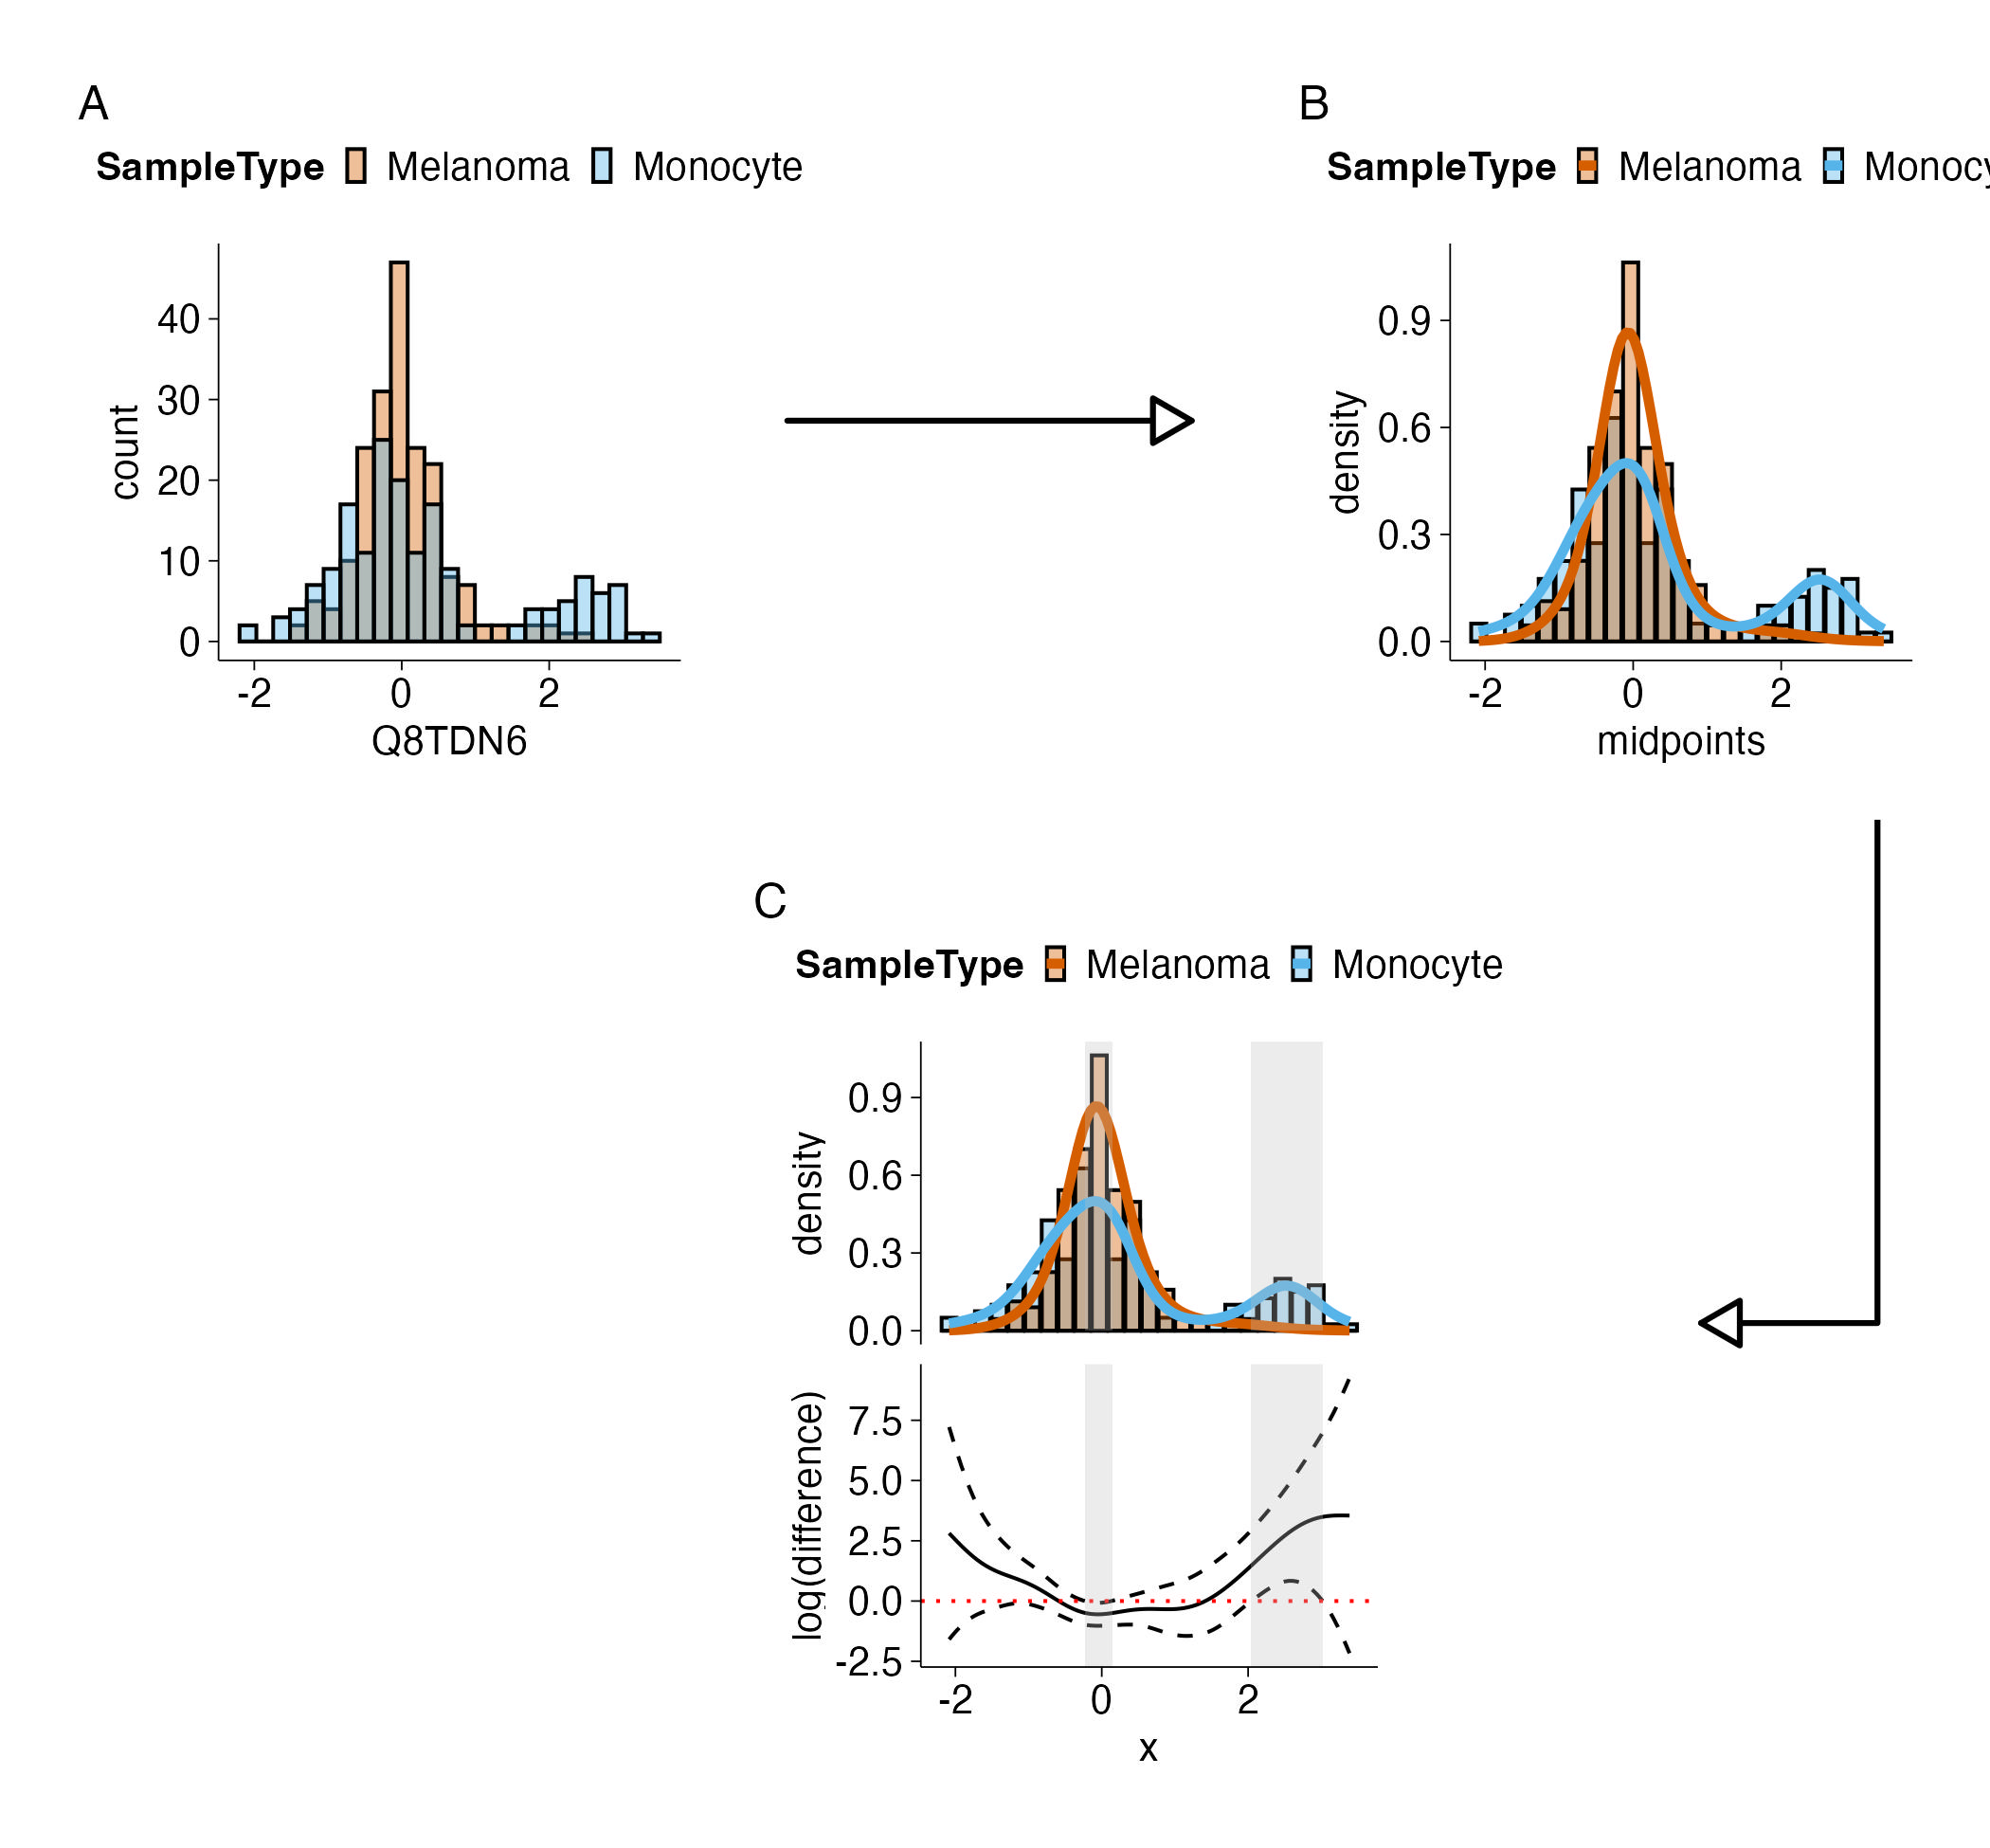
\includegraphics[width=0.85\linewidth]{figs/fig2.jpg}
    \caption{\textbf{Overview of the gamdid workflow} The complete workflow for fitting GAMs to compare distributions is illustrated using a ribosome biogenesis protein from the Leduc dataset. \textbf{A}: Raw protein abundance values are discretized into histogram bin counts, recasting the density estimation problem as Poisson regression. This representation preserves distributional shape information that is lost in a mean-based summary. \textbf{B}: A Poisson generalized additive model (GAM) is fitted to the bin counts as a function of bin midpoints, allowing each group (melanoma and monocyte) to have its own flexible, non-parametric density curve. The GAM framework accommodates any distributional shape without parametric assumptions. \textbf{C} (top): The fitted density curves generated by gamdid's visFit function, with gray shading highlighting regions where the distributions differ significantly between groups. \textbf{C} (bottom): The difference smoother representing the log-ratio of densities between groups along with its simultaneous confidence band. Regions where this band excludes zero identify statistically significant local distributional differences, linking inference to an interpretable visualization. This combination of flexible modeling, hypothesis testing, and interpretable visualization is an innovative feature unique to gamdid.}
    \label{fig:workflow}
\end{figure}

This representation allows for density estimation through Poisson generalized additive models, where expected counts are modeled as a function of the bin midpoints and by specifying a group-specific spline, each group has its own unique density shape. The GAM fits are displayed in Figure \ref{fig:workflow} panel B.

Inference is subsequently carried out using the GAM framework, with differences between groups assessed using Wald-type tests by comparing group-specific model parameters. This yields a p-value for inferring any type of distributional difference both in location and in shape, referred to as the GAM p-value in the remainder of the manuscript.\\
To increase the power to detect distributional changes that are strongly driven by differences in the mean, the p-value obtained from the GAM is combined with a p-value derived from the \texttt{msqrob2} framework, a conventional mean-based approach for DA analysis \cite{msqrob}. The two p-values are integrated using the harmonic mean p-value (HMP) method \cite{harmonicp}.
This results in a final aggregated p-value for each feature, providing a single, robust measure of evidence for any distributional change.

Interestingly, \texttt{gamdid} also provides an interpretable visualization that is directly linked to the inference, by constructing a difference smoother along with a simultaneous confidence band. Regions where this band does not include zero indicate a statistically significant local distributional difference, as illustrated in Figure \ref{fig:workflow} panel C.
%Note However that pinpointing differential regions in the distribution is not possible for all features, sometimes no specific region is significant enough to fall out of the confidence band.
\subsection{Simulation study for benchmarking}
To benchmark \texttt{gamdid} for single cell proteomics applications, we constructed semi-synthetic simulations based on two publicly available mass spectrometry (MS)-based SCP data sets obtained from the R/Bioconductor package \texttt{scpdata} \cite{scp_paper}: the TMT-labeled single-cell Leduc dataset \cite{leduc} consisting of 1531 cells and 6706 identified peptides, and the label-free single-cell Petrosius dataset \cite{petro} consisting of 564 cells and 5729 identified peptides.\\
For each dataset, preprocessed (see Methods) protein-level summarized assays from one cell type were selected and the corresponding cells were randomly assigned to two mock groups (A and B). Hence, all proteins are non-DD between A and B.\\
Only proteins with at least 50 non-missing observations per group were retained for benchmarking, consistent with the default setting in the \texttt{gamdid} package. This threshold ensures a sufficient number of observations to reliably characterize the distribution of each feature, as fewer observations may yield an incomplete or misleading representation of the underlying density.
\\
\\
\textbf{Simulation of distributional differences}
Following the framework established by Korthauer et al. (2016) \cite{scdd}, we introduced five categories of distributional differences by altering protein abundances in cells of group B: differential expression (DE) (a pure mean shift, which corresponds to DA), differential variability (DV), \textcolor{red}{differential both in modality and component means} (DB), differential modality (DM), and differential proportion (DP), as illustrated in Figure \ref{fig:diffsim}. These effects were introduced in 20\% of randomly selected features by systematic shifting of the abundances in subsets of the cells in group B (for the DE, DB, DM and DP scenarios) or by adding controlled random noise (for the DV scenario).

\begin{figure}[H]
    \centering
    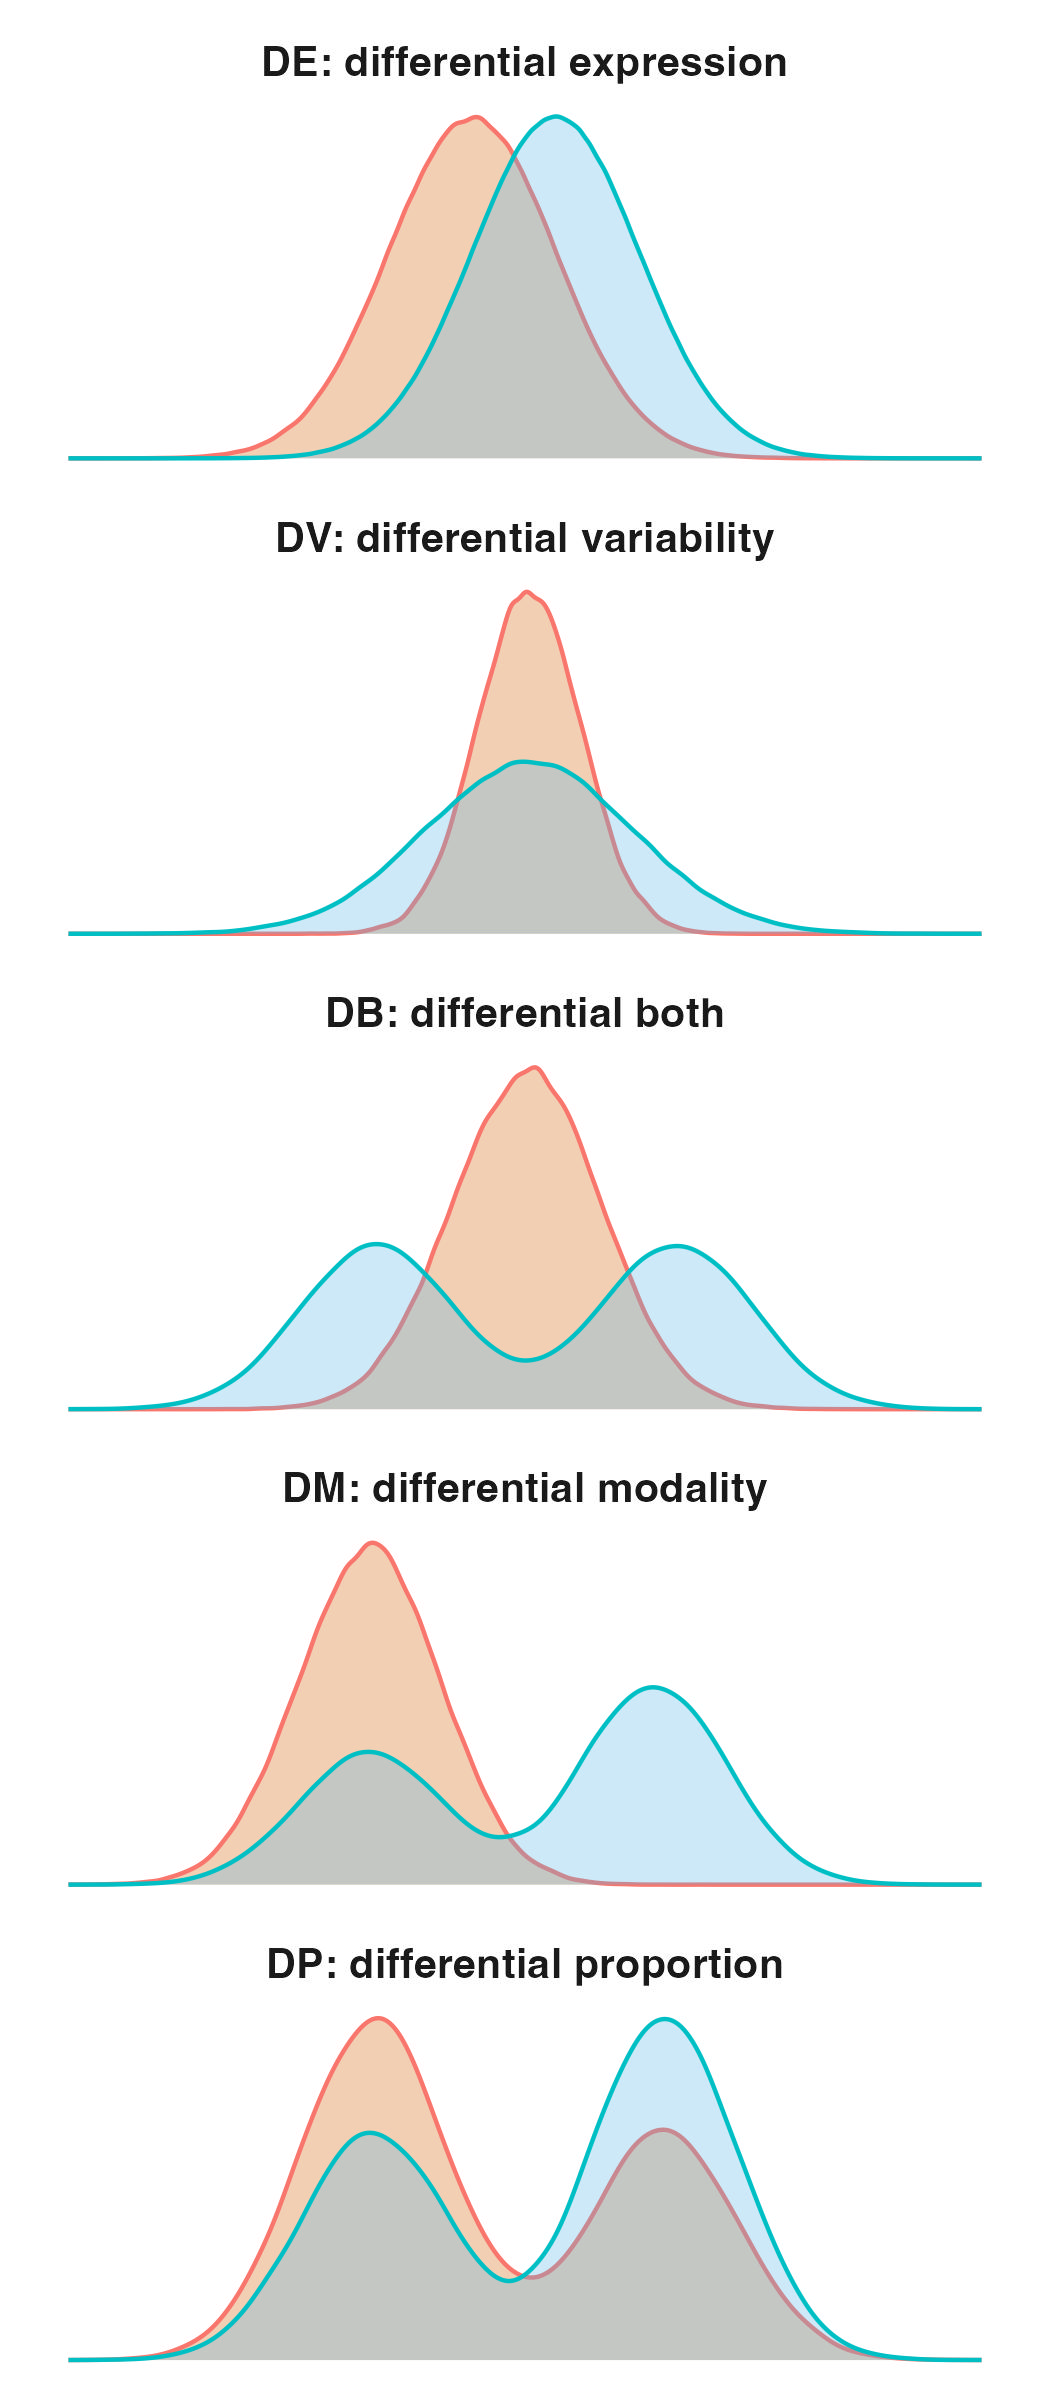
\includegraphics[width=0.425\linewidth]{figs/fig3.jpg}
    \caption{\textbf{Five simulation scenarios used to benchmark gamdid} To evaluate gamdid's ability to detect different types of distributional differences, five categories of signal, established by Korthauer et al. (2016) \cite{scdd}, were introduced into real single-cell proteomics data. \textcolor{red}{DE:} a pure shift in the mean, equivalent to conventional DA. \textcolor{red}{DV:} an increase in variance without a location shift, reflecting e.g. heterogeneous cellular responses. \textcolor{red}{DB:} a bimodal distribution induced in one group by shifting subsets of cells in opposite directions, without altering the overall mean. \textcolor{red}{DM:} an asymmetric shift in one tail, creating a difference in skewness or the emergence of a subpopulation. \textcolor{red}{DP:} a change in the relative weight of a subpopulation shared between groups.}
    \label{fig:diffsim}
\end{figure}

This semi-synthetic approach leverages real SCP data rather than fully synthetic 'clean' simulations, and thus preserves realistic distributional characteristics inherent to single-cell proteomics measurements.
\\
\\
\textbf{Method comparison}
We compare \texttt{gamdid} to \texttt{distinct} as the primary benchmark method. \texttt{BASiCS} and \texttt{scDD} were excluded from the comparison as \texttt{BASiCS} is limited to detecting shifts in mean and variance, and therefore cannot be applied to the majority of the simulations, while \texttt{scDD} requires count data as input, which is incompatible with the continuous abundance measurements obtained in proteomics data.

\texttt{distinct} performs group comparisons by computing the average difference between empirical cumulative distribution functions (ECDFs) and can optionally account for subgroup structure in multi-sample multi-cell designs. As our datasets, similar to most public SCP datasets, do not have these multi-sample multi-cell designs, \texttt{distinct} was applied without this option.\\
Note that the current implementation of \texttt{gamdid} does not account for subgroup structure.\\
Method performance is evaluated using false discovery proportion — true positive proportion (FDP-TPP) curves. For a given significance threshold, the FDP represents the proportion of false positives among all features called significant, while the TPP represents the proportion of true positives recovered out of all truly differential features. An FDP-TPP curve allows one to assess the power of a method (TPP) at any given level of false discoveries (FDP). This provides a more complete picture of method performance than a single summary statistic, and allows for a direct visual comparison of the trade-off between sensitivity and false discovery control across competing methods. A method can be considered more powerful when the area under its FDP-TPP curve is larger. The dashed vertical line at FDP = 0.05 serves as a reference for the nominal FDR threshold.
\\
\\
\textbf{GAM evaluation}
We first evaluate the performance of the GAM methodology in isolation (without p-value aggregation via \texttt{msqrob2}) against \texttt{distinct}. \textcolor{red}{The FDP-TPP curves for both datasets are presented in Figure \ref{fig:leducsims_gam}.}

The GAM method demonstrates conservative false discovery rate control and exhibits substantially superior performance compared to \texttt{distinct} when distributional changes do not involve shifts in mean (DV and DB scenarios). Conversely, in the scenarios where mean shifts contribute to the distributional change, \texttt{distinct} outperforms the GAM method and is even on par with conventional DA analyses like \texttt{msqrob2}. This observation motivated the aggregation of GAM-derived p-values with \texttt{msqrob2} p-values, thereby combining the GAM methodology's sensitivity to differences in shape with \texttt{msqrob2}'s established performance for detecting mean shifts.

\begin{figure}[H]
    \centering
    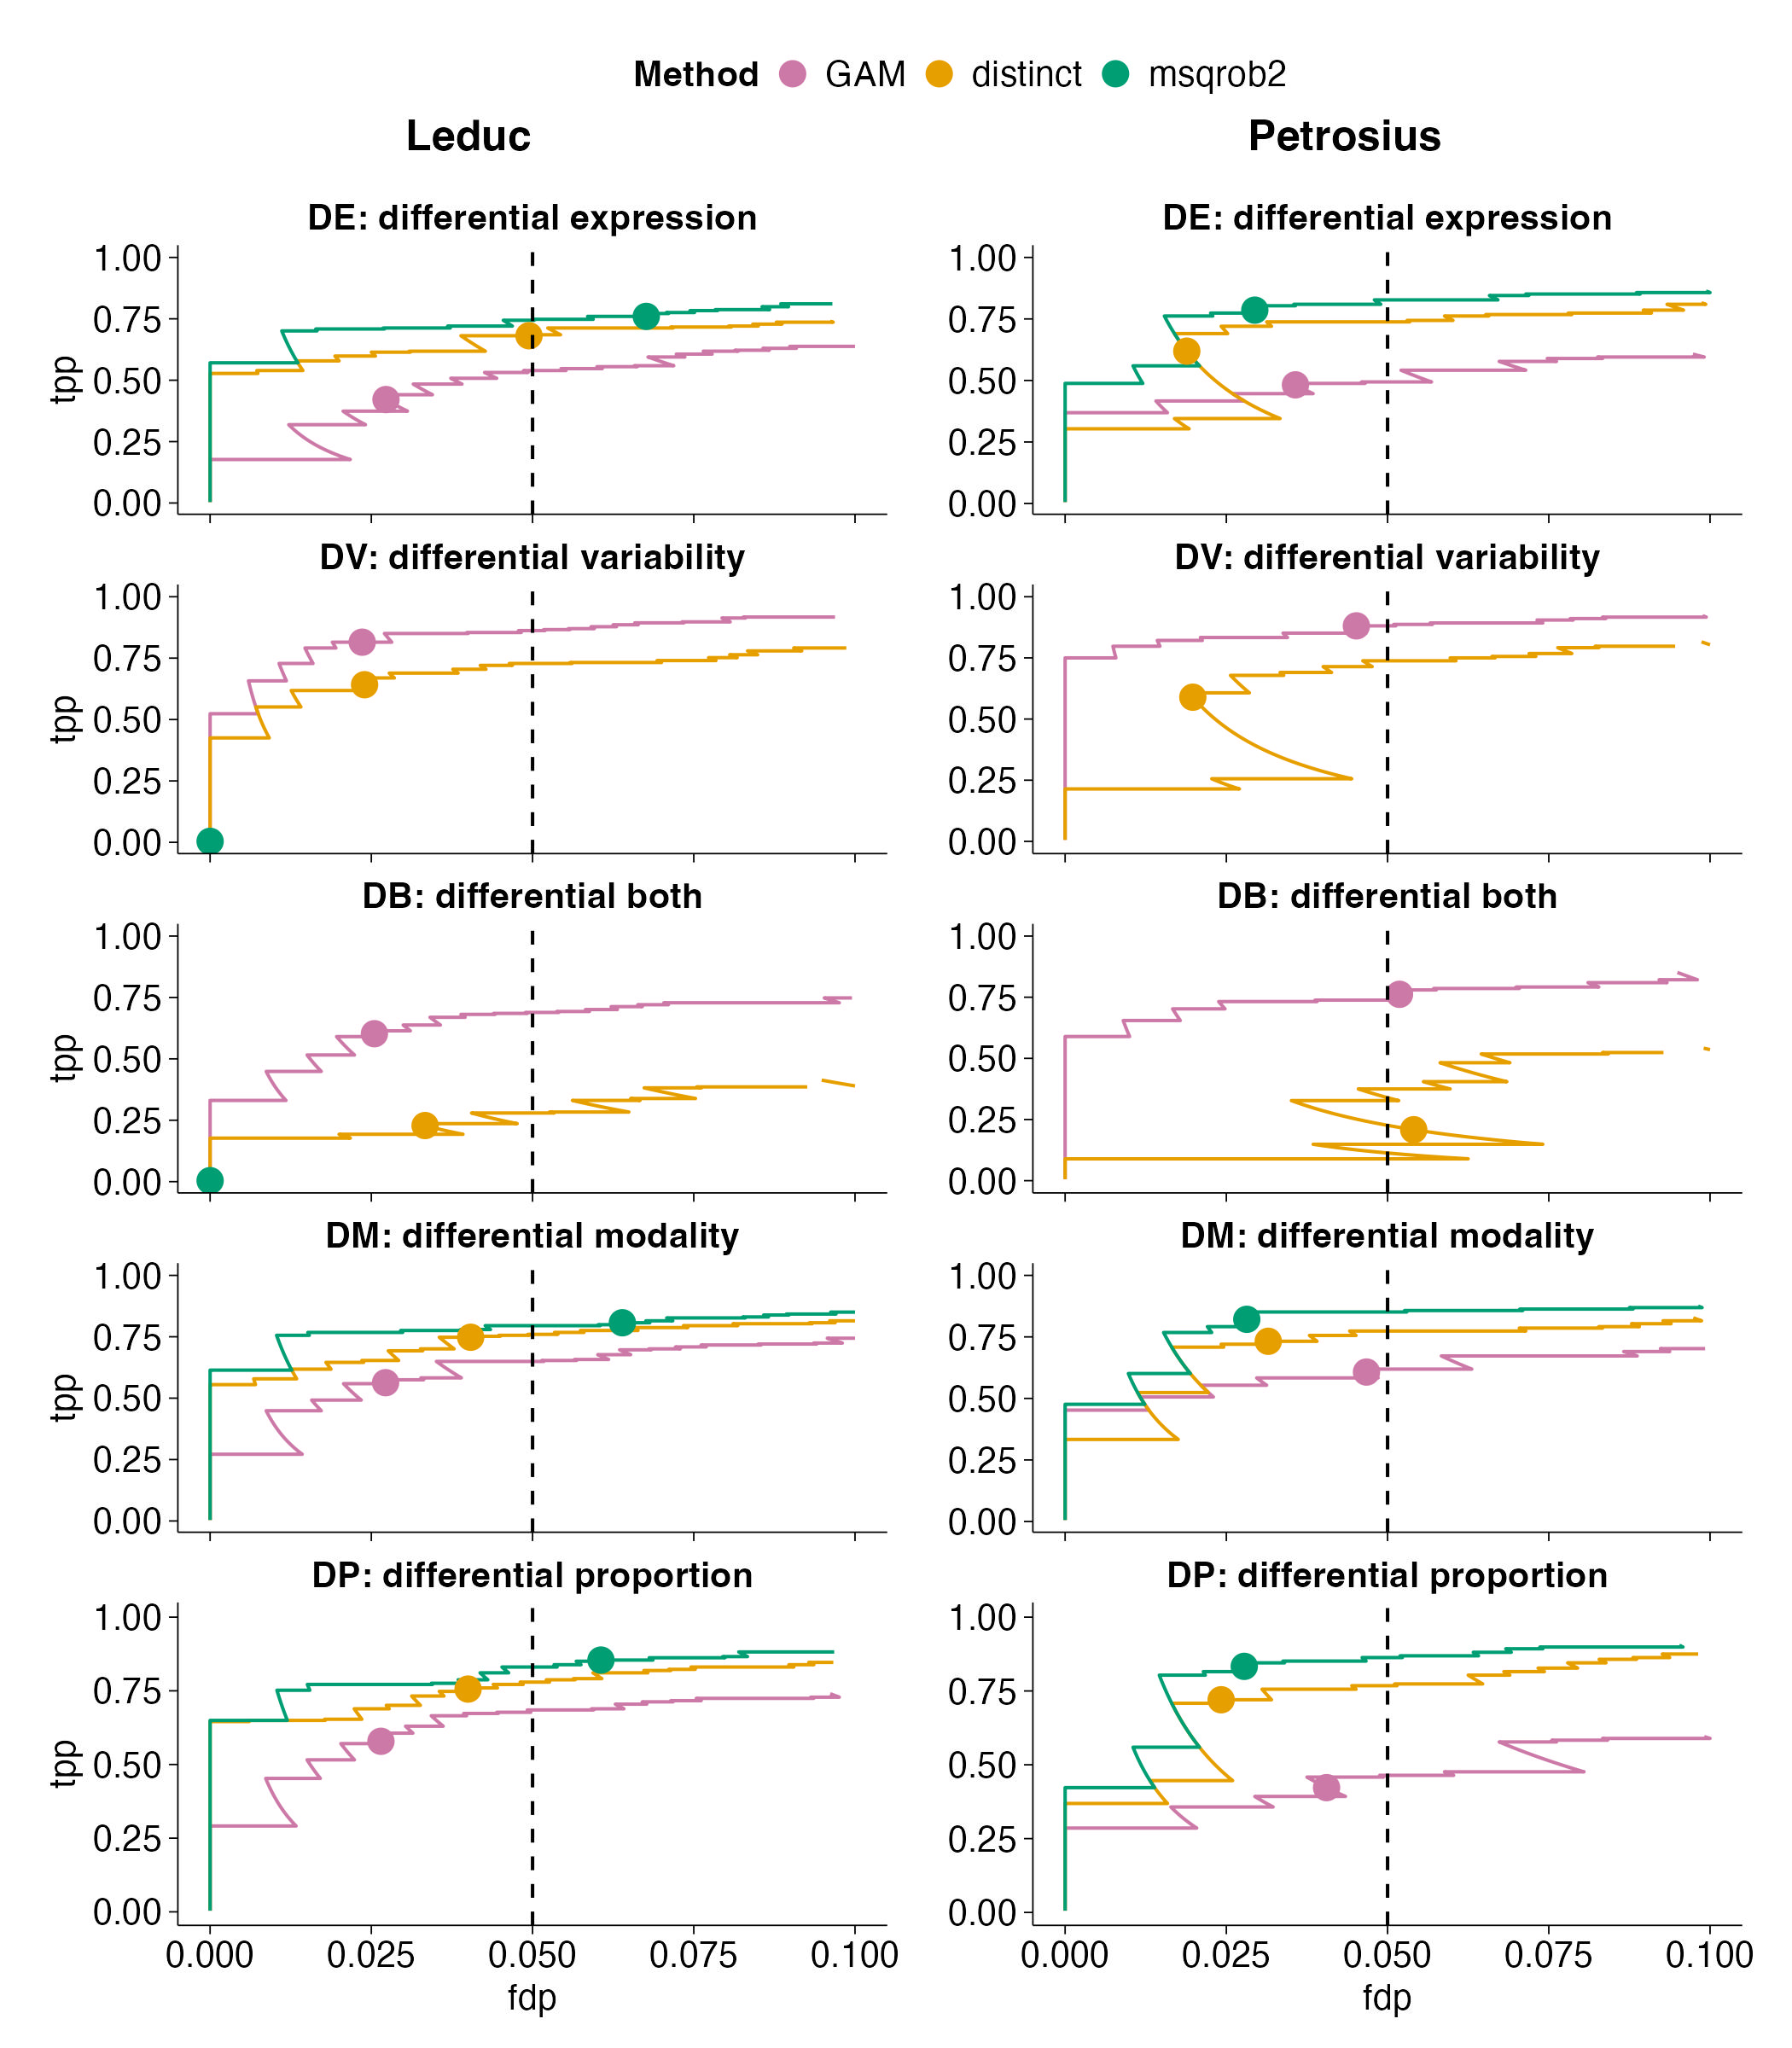
\includegraphics[width=0.85\linewidth]{figs/fig4.jpg}
    \captionsetup{labelfont={bf,small,color=red}}
    \caption{\textbf{\textcolor{red}{Performance of the standalone GAM method}} FDP-TPP curves comparing the standalone GAM method, msqrob2, and distinct across the five simulation scenarios, based on the protein-level mock data of the Leduc dataset (left; 755 monocytes) and the Petrosius dataset (right; 269 m2i cells). Each curve traces the trade-off between TPP (sensitivity) and FDP as the significance threshold is varied; the dots mark the 5\% FDR threshold and the dashed vertical line marks FDP = 0.05. The GAM method achieves conservative FDR control. For distributional changes that do not involve a mean shift (DV, DB), the GAM method substantially outperforms distinct in both datasets, demonstrating its superior sensitivity to shape differences. However, for scenarios where mean shifts contribute to the distributional change (DE, DM, DP), distinct and msqrob2 outperform the standalone GAM method. This complementarity motivates the aggregation of GAM p-values with msqrob2 p-values in the gamdid pipeline. Notably, improvements of the GAM method over distinct are more pronounced in the Petrosius dataset,
which is attributable to the smaller sample size: contrary to gamdid, distinct relies on permutation-based inference and suffers from
reduced null distribution resolution with fewer observations. DB (differential both) denotes a difference in both modality and component means.}
    \label{fig:leducsims_gam}
\end{figure}


\textbf{gamdid evaluation}
Figure \ref{fig:leducsims_gamdid} presents the FDP-TPP curves comparing \texttt{distinct} and \texttt{gamdid} for both datasets. The corresponding numbers of true and false positives at the 5\% FDR threshold are also provided in the supplementary materials (Figures \ref{fig:TP} and \ref{fig:FP}): \texttt{gamdid} recovers a comparable or larger number of true positives, while the false positives are similarly low for both methods.
\texttt{gamdid}'s performance is comparable to \texttt{distinct} for pure mean shifts (DE), shows modest improvements for distributional changes that involve location shifts (DM, DP), and shows substantial improvements for distributional changes in shape (DV, DB).

Improvements are more pronounced in the Petrosius simulations, which could be attributable to the smaller sample size in the Petrosius dataset compared to Leduc.
To examine this, we subsampled the Leduc dataset such that the average number of non-missing observations per group over all features matched that of the Petrosius dataset. The resulting FDP-TPP curves are provided in the supplementary materials in Figure \ref{fig:leducsims_gamdid_subsample}. Indeed, the improvements are more pronounced in the subsampled simulations compared to the Leduc simulations in Figure \ref{fig:leducsims_gamdid}. This supports the hypothesis that \texttt{gamdid} exhibits higher power under smaller sample conditions compared to \texttt{distinct}, which suffers from a reduced resolution of the null distribution due to a limited number of permutations.

\begin{figure}[H]
    \centering
    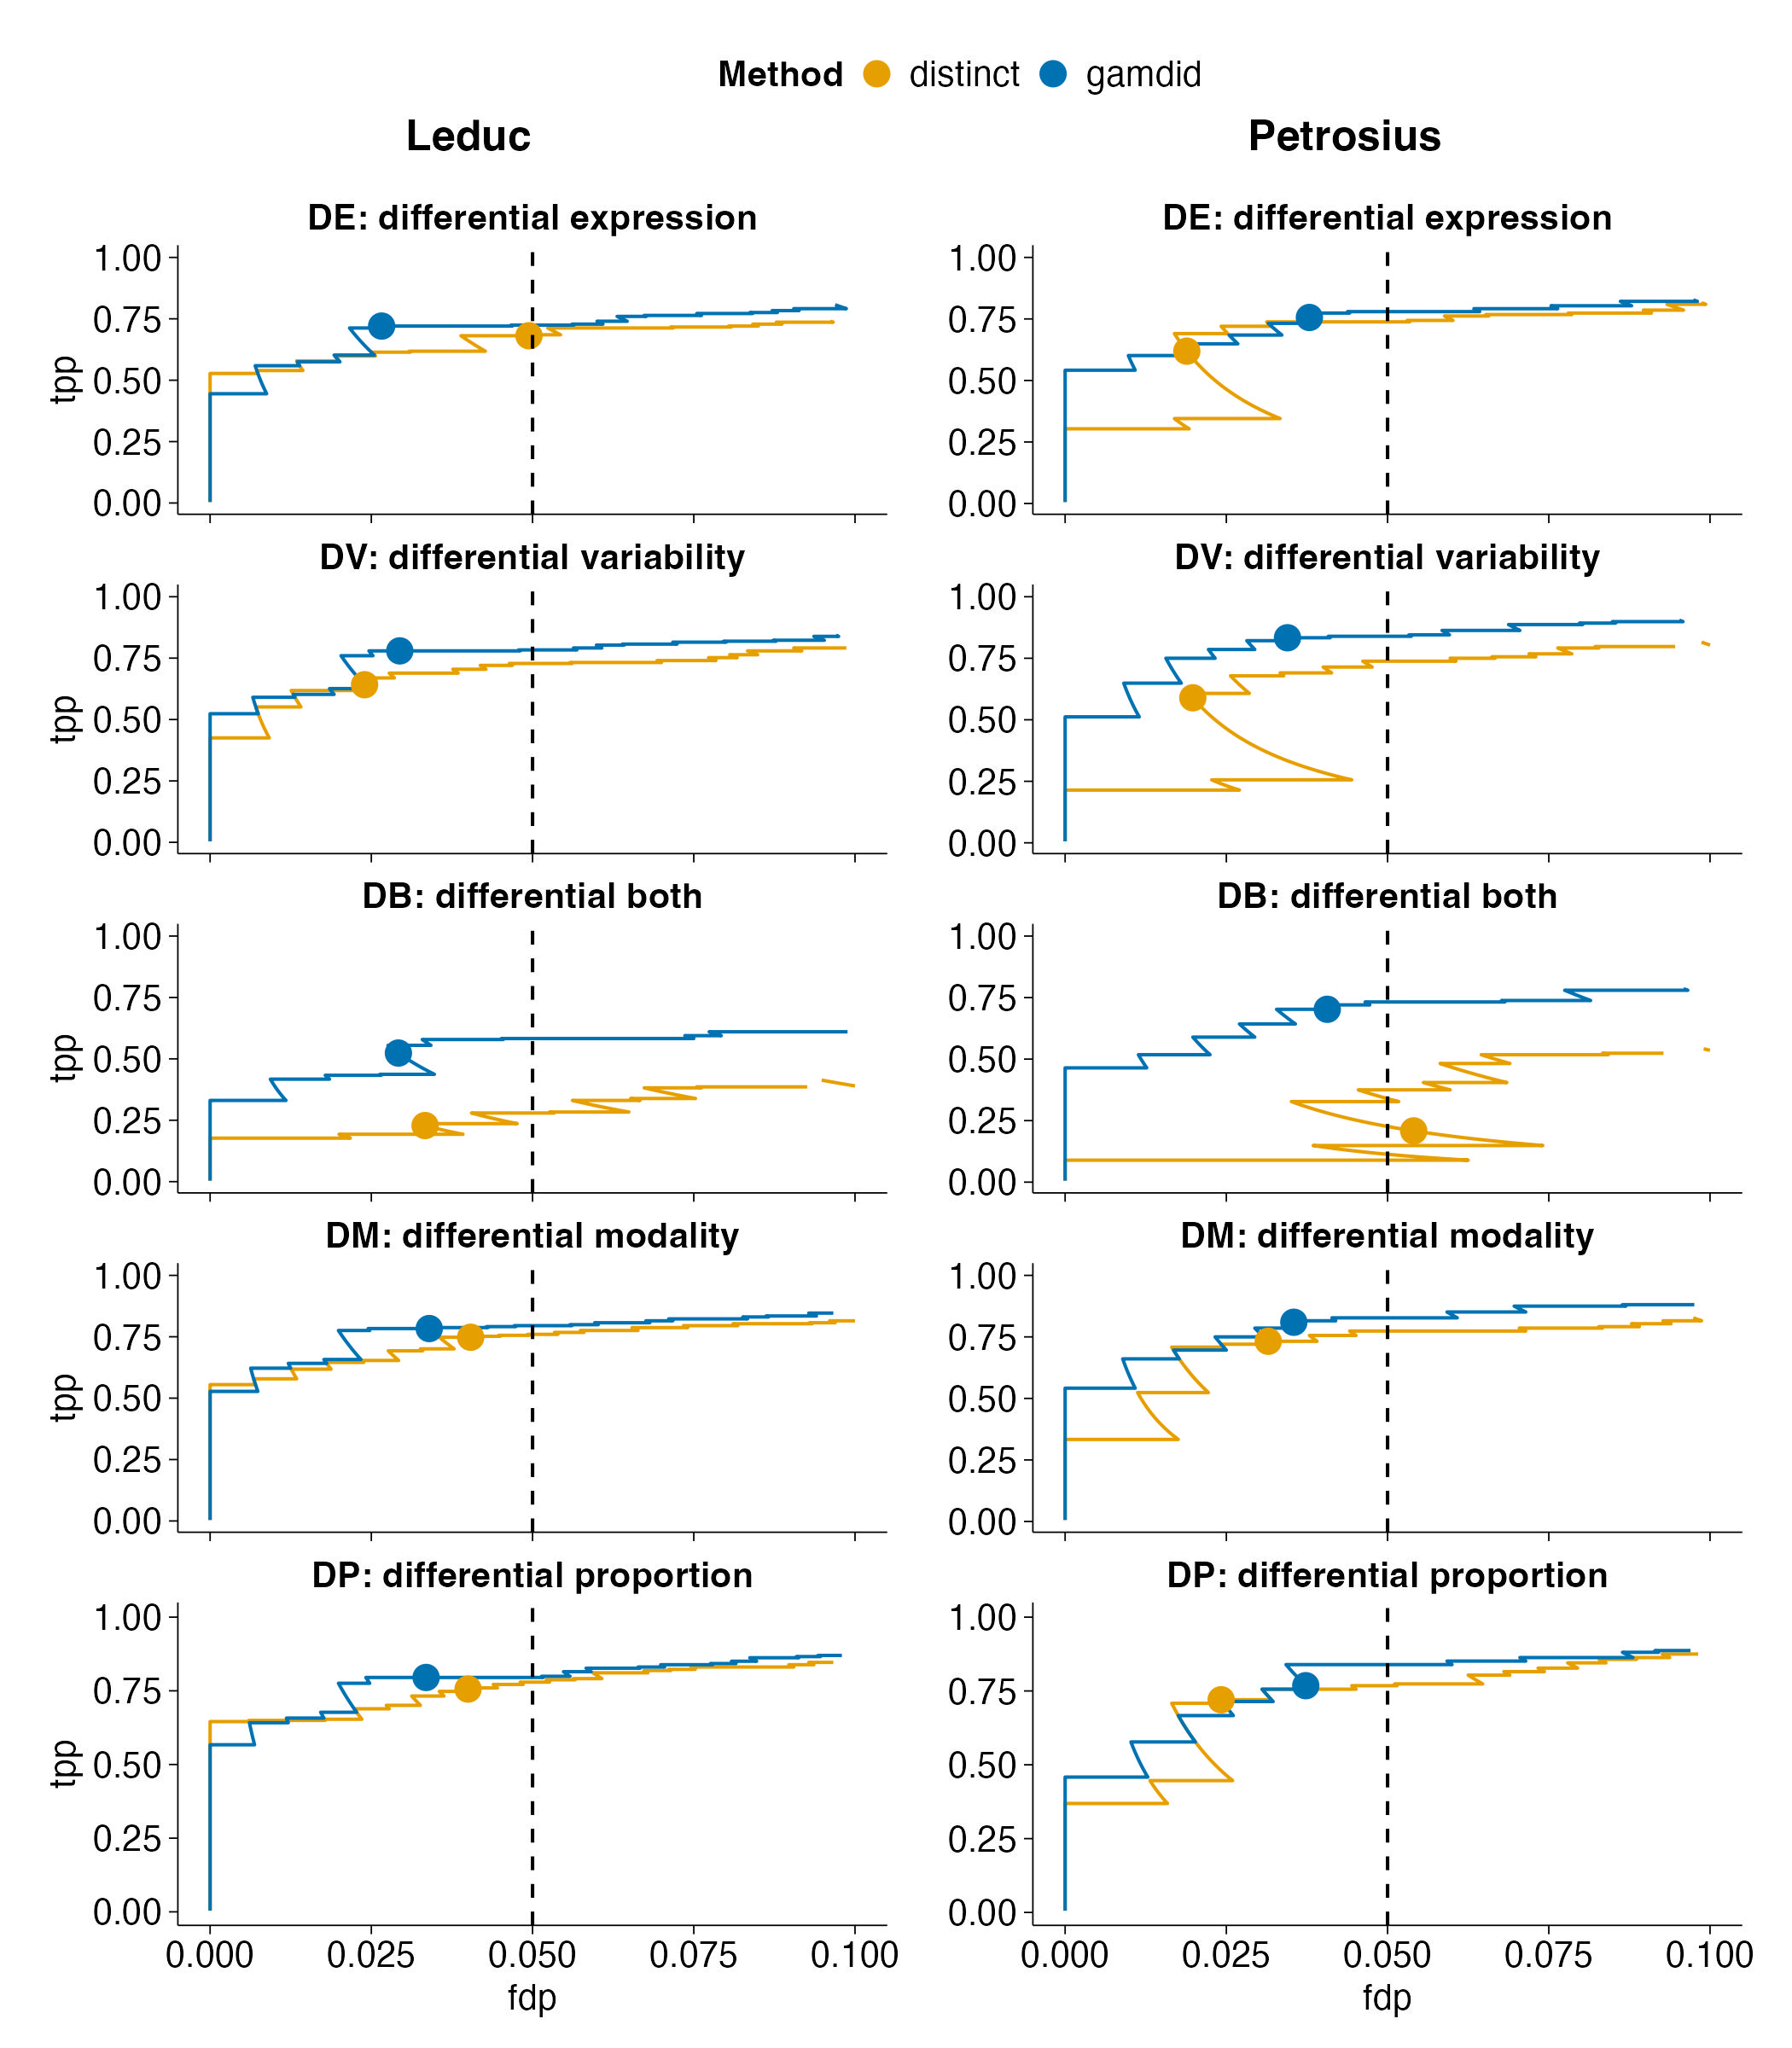
\includegraphics[width=0.85\linewidth]{figs/fig5.jpg}
    \captionsetup{labelfont={bf,small,color=red}}
    \caption{\textbf{\textcolor{red}{Performance of gamdid}} FDP-TPP curves comparing the gamdid method (combining GAM and msqrob2 p-values via the harmonic mean p-value) against distinct across the five simulation scenarios, based on the protein-level mock data of the Leduc dataset (left; 755 monocytes) and the Petrosius dataset (right; 269 m2i cells). The dots mark the 5\% FDR threshold and the dashed vertical line marks FDP = 0.05. By combining the local density sensitivity of the GAM with the established power of msqrob2 for mean shifts, gamdid achieves performance that is comparable to distinct for pure mean shifts (DE), shows modest improvements for distributional changes that involve a location component (DM, DP), and demonstrates substantial improvements for pure shape changes (DV, DB). gamdid maintains conservative FDR control throughout. These results demonstrate that p-value aggregation successfully bridges the complementary strengths of both components, yielding a single method competitive across the full spectrum of distributional differences. DB (differential both) denotes a difference in both modality and component means.}
    \label{fig:leducsims_gamdid}
\end{figure}




To assess the robustness of the conclusions under less pronounced distributional differences, FDP-TPP curves for simulations with 25\% reduced signal magnitudes are provided in the supplementary materials (Figure \ref{fig:leducsims_lower_gamdid}). These results are consistent with the findings above, indicating robust performance.

\textbf{Interpretation and visualization}
In contrast to competing methods, \texttt{gamdid} provides informative visualizations of features picked up as DD. Figure \ref{fig:DV_example} illustrates this functionality for a significant feature identified under the DV simulation framework. This visualization integrates GAM fits with highlighted differential regions, providing immediate visual evidence of differential variability between groups.

\begin{figure}[H]
    \centering
    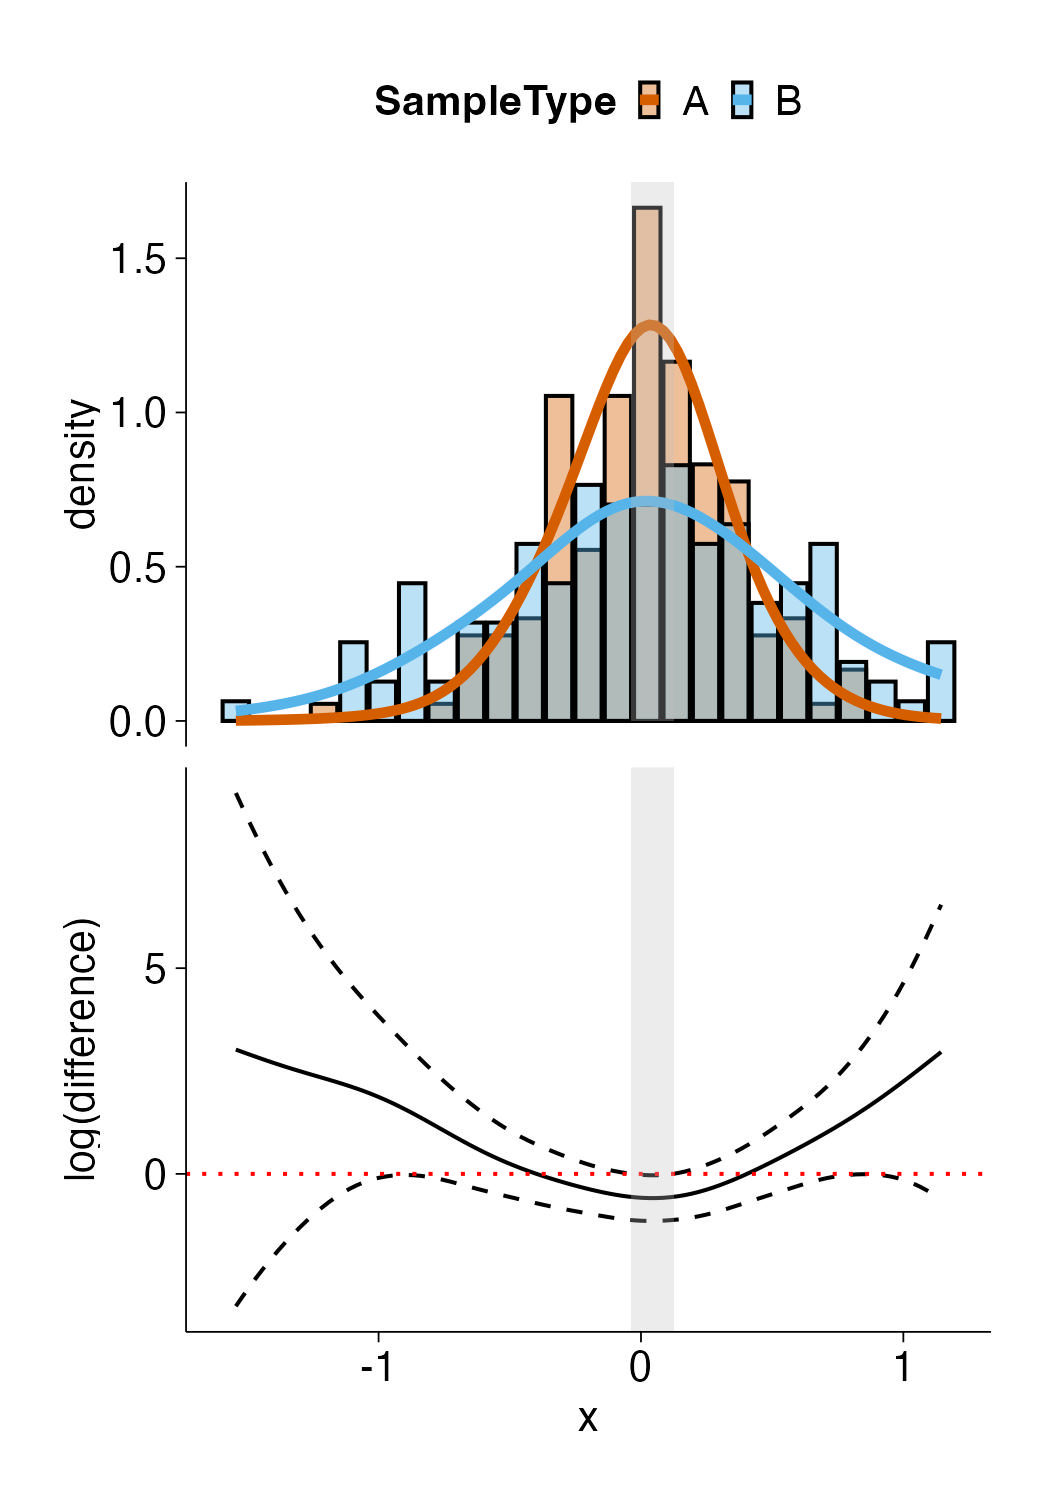
\includegraphics[width=0.425\linewidth]{figs/fig6.jpg}
    \caption{\textbf{gamdid's interpretable visualization for a DV-simulated feature in the Petrosius dataset} A feature with induced differential variability (DV simulation), visualized using gamdid's visFit function. The top panel shows the fitted GAM density curves for both groups, overlaid on the observed histograms. The bottom panel displays the difference smoother (log-ratio of densities) along with its simultaneous confidence band; the gray-shaded region identifies the specific abundance range where the distributional difference is statistically significant. Unlike competing DD methods such as distinct, gamdid does not merely return a p-value; this visualization provides immediate visual evidence of differential variability between groups.}
    \label{fig:DV_example}
\end{figure}


\textbf{Peptide-level simulations}
The same simulation framework was applied to peptide-level assays for both the Leduc and Petrosius datasets. The resulting FDP-TPP curves are provided in the supplementary materials in Figure \ref{fig:leducsims_pep} and are consistent with the protein-level results.\\
Note, however, that the FDR control at the nominal 5\% threshold is less conservative at the peptide level due to the correlation structure inherent to peptide-level data, a well-known challenge in peptide-level analyses. Nevertheless, this demonstrates that \texttt{gamdid} provides a flexible framework suitable for inferring DD at different quantification levels (precursor, peptide, protein) in MS-based proteomics data.
\\
\\
\textbf{Three-group simulations}
A unique advantage of \texttt{gamdid} is its support for omnibus testing across more than two groups, followed by post-hoc pairwise comparisons corrected for multiple testing using the stagewise testing procedure \cite{stagewise_testing}. The omnibus test simultaneously assesses whether any distributional difference exists between any  of the groups. No competing DD analysis method currently offers this functionality.\\
To evaluate this functionality, we extended the simulation framework described above to a three-group setting, randomly assigning cells to mock groups A, B, and C, with distributional signal introduced in group B under the same five simulation scenarios as above. The omnibus test was applied to this three-group comparison and the resulting FDP-TPP curves are provided in the supplementary materials in Figure \ref{fig:leduc_threegroup}. Note that, as none of the competing DD methods supports multi-group testing, a formal benchmark comparison is not possible here.\\
Interestingly, the three-group setting yields higher power than the two-group comparison under equal signal strength. Note that this might arise from the default minimum observation requirement of 50 cells per group imposed by \texttt{gamdid}, which, in the three-group analysis, requires more observations than in the two-group analysis, leading to more powerful inference.
\subsection{Case study}
We next illustrate the utility of \texttt{gamdid} in a case study based on the Leduc dataset.\\
First, we randomly divide the monocyte cells into two mock groups: X (containing 377 cells) and Y (containing 378 cells). In group Y, we spike in 10\% of the 697 sub-cluster A melanoma cells (69 cells) to simulate a subpopulation in group Y.\\
Figure \ref{fig:volanoPlots} shows the volcano plot of the conventional DA \texttt{msqrob2} analysis twice. In panel A, significant features of the DA analysis are marked in red, while in panel B the significant features of DD methods \texttt{gamdid} and \texttt{distinct} are marked.

\begin{figure}[H]
    \centering
    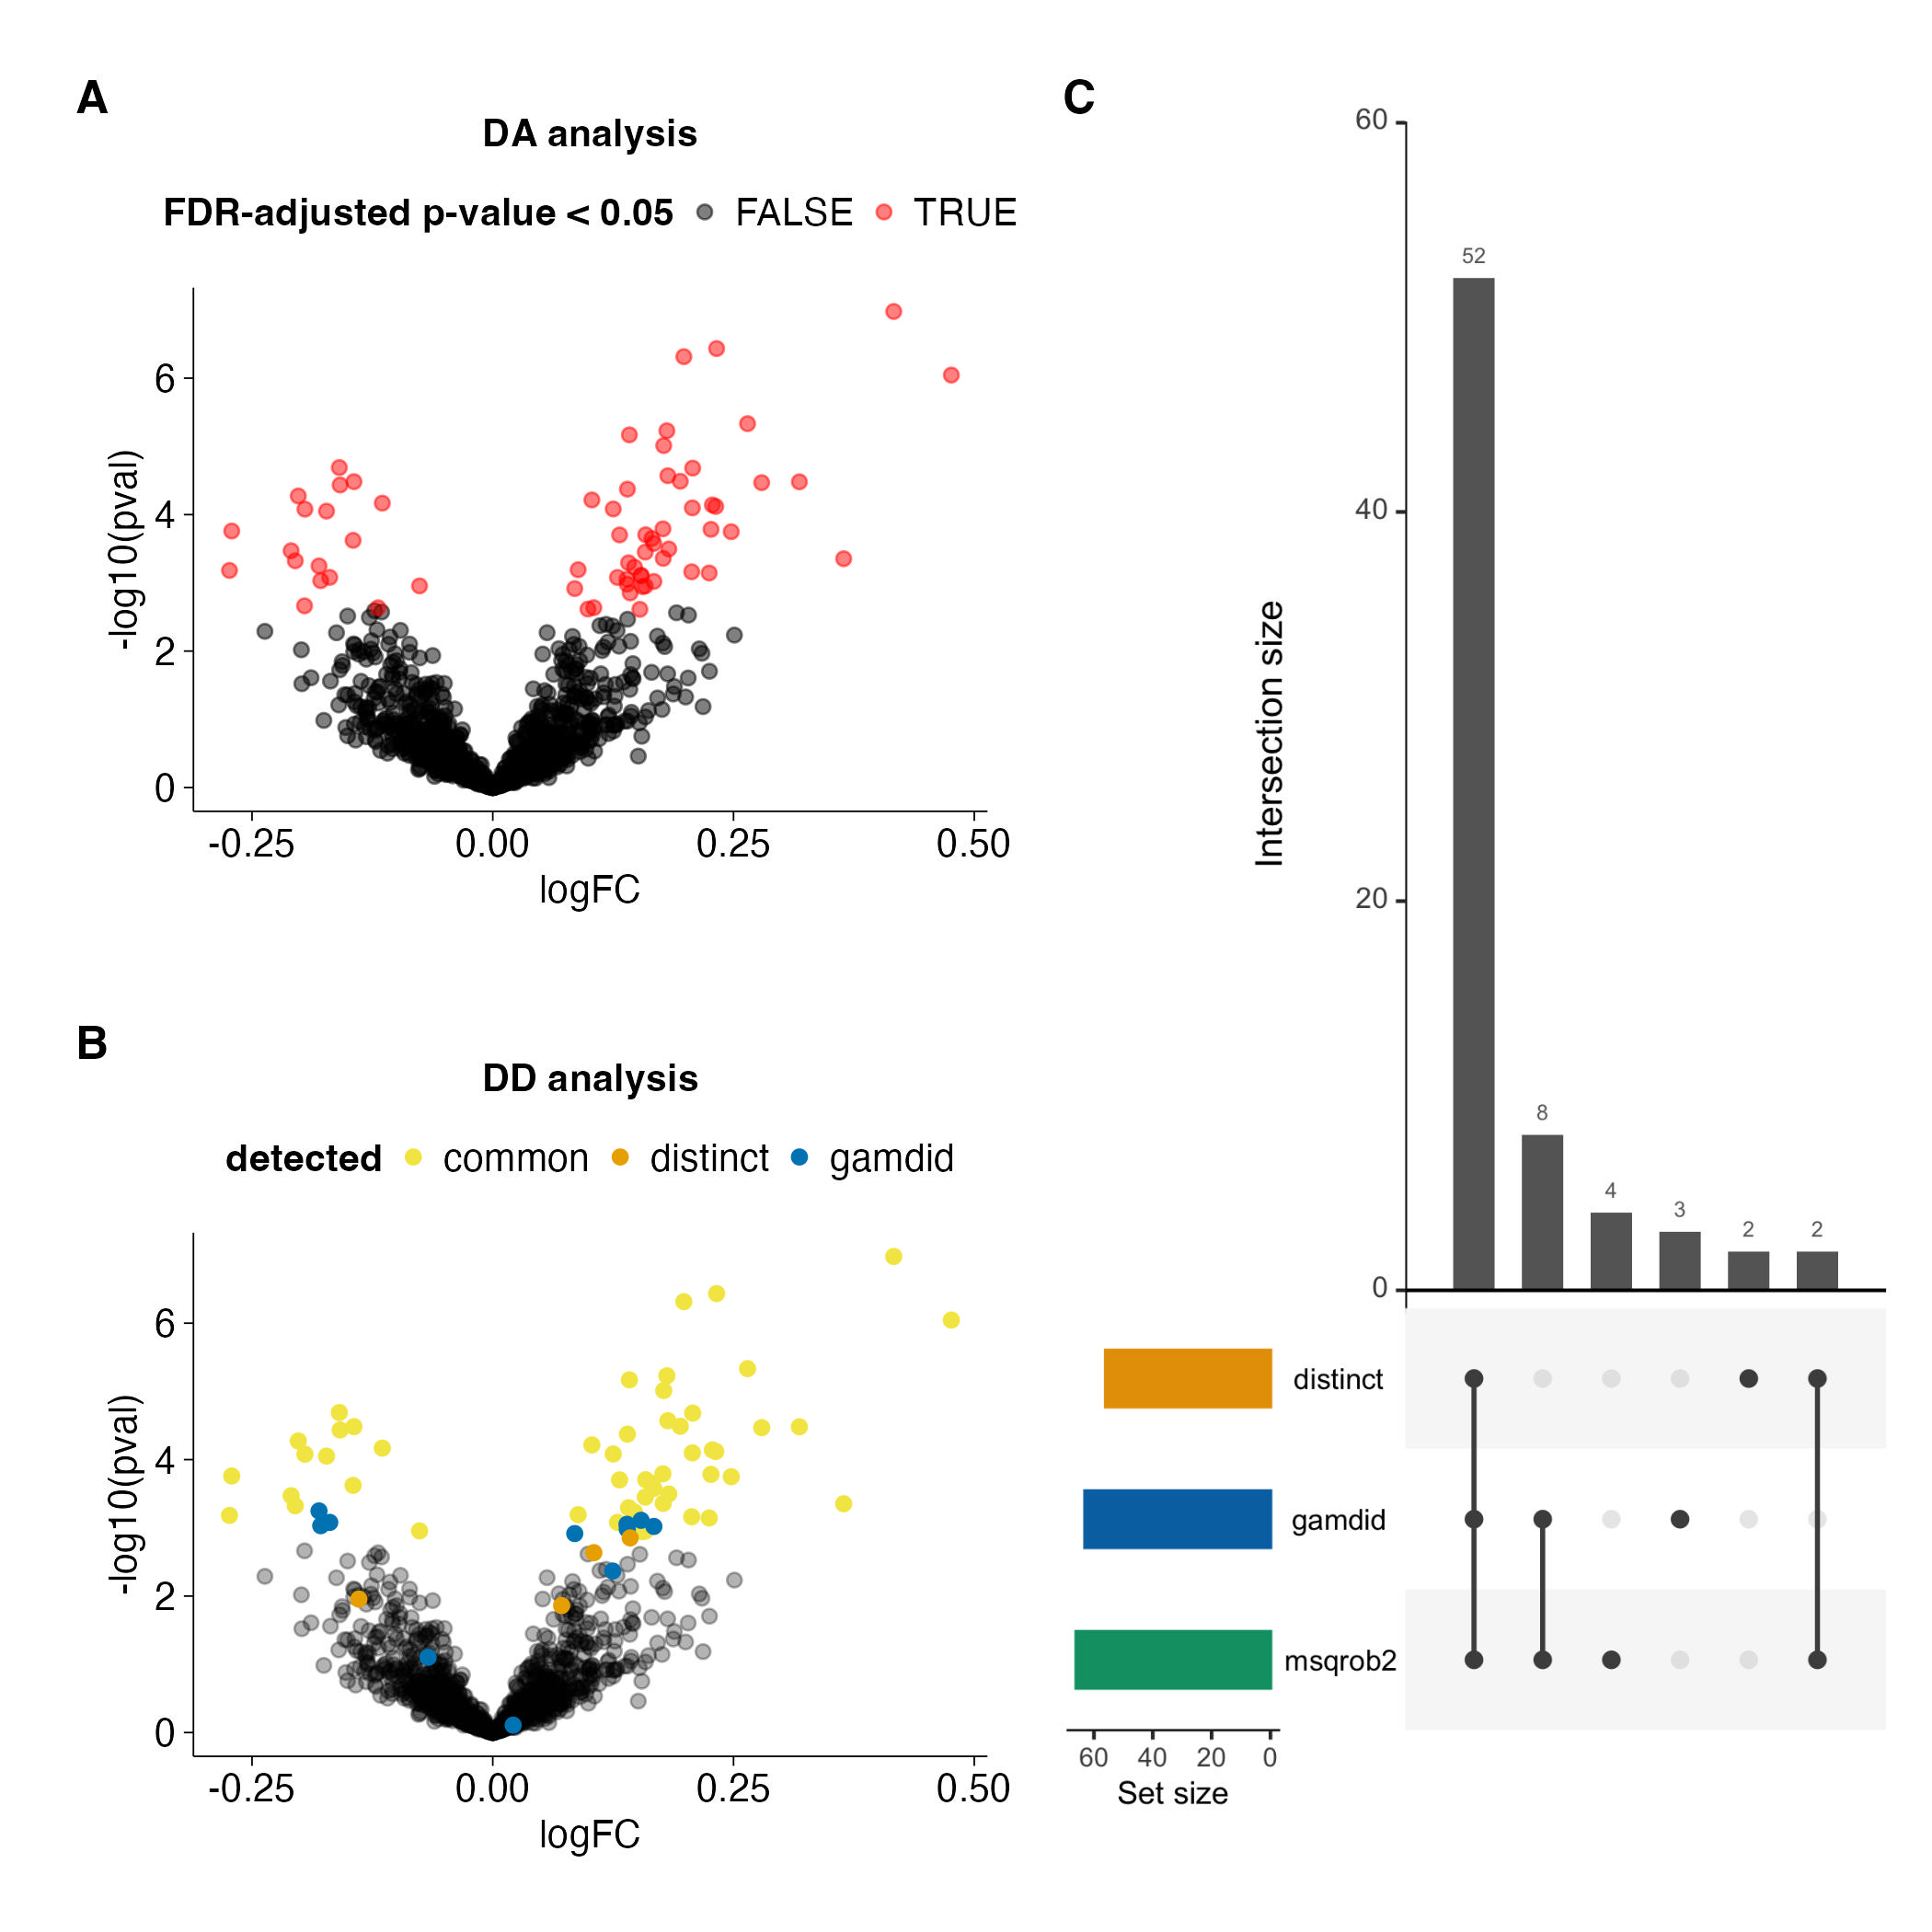
\includegraphics[width=0.85\linewidth]{figs/fig7.jpg}
    \captionsetup{labelfont={bf,small,color=red}}
    \caption{\textbf{\textcolor{red}{Case study: gamdid detects distributional changes missed by conventional DA analysis}} A controlled spike-in experiment based on the Leduc dataset: monocyte cells are split into two mock groups (X: 377 cells; Y: 378 cells), and 10\% of the 697 sub-cluster A melanoma cells (69 cells) are spiked into group Y to simulate the emergence of a subpopulation. Panels A and B display the same msqrob2 volcano plot. \textbf{A}: Features found significant by conventional DA (msqrob2) are highlighted in red. \textbf{B}: The same volcano plot, now colored by DD method detection: yellow = detected by both distinct and gamdid; orange = detected by distinct only; blue = detected by gamdid only. Both DD methods detect the majority of DA features, while also prioritizing some features missed by conventional DA methods. \textbf{C}: UpSet plot showing the overlap in significant features between distinct, gamdid and msqrob2. The horizontal bars (left) show the total number of significant features per method (Set size); the vertical bars (top) show the size of each intersection, with the dot matrix below indicating which methods contribute to each intersection. The six features picked up by msqrob2 and missed by gamdid are borderline significant for msqrob2 and borderline non-significant for gamdid (this is not the case for distinct, see Table \ref{tab:only_msqrob2}), which means that only gamdid largely preserves the ranking of DA features. Moreover, gamdid prioritizes three features that are missed by both msqrob2 and distinct (see Table \ref{tab:only_gamdid}).}
    \label{fig:volanoPlots}
\end{figure}

Figure \ref{fig:volanoPlots}C presents a method comparison for
the significant features in the spike-in case study. Overall, the methods produce
similar results with 52 features found significant by all three.


Only six features are picked up by \texttt{msqrob2} and missed by \texttt{gamdid}.
These features are borderline significant for \texttt{msqrob2} and borderline
non-significant for \texttt{gamdid}, which is illustrated in table
\ref{tab:only_msqrob2} in supplementary materials.\\
Furthermore, \texttt{gamdid} prioritizes three features that \texttt{msqrob2}
and \texttt{distinct} fail to detect (see Table \ref{tab:only_gamdid} in
supplementary materials).
Interestingly, even features detected by all three methods illustrate the utility
of \texttt{gamdid}. Figure \ref{fig:caseStudy_exs} shows the
\texttt{gamdid} visualization for four representative features (panels A--D), displaying the
mock groups (top) and the spike-in study (middle). The boxplot at the bottom of each panel
indicates where the spiked-in melanoma cells are
located within the distribution of group Y. Figure \ref{fig:caseStudy_exs} clearly
shows that these features are DD due to the subpopulation of spike-in cells rather
than DA. Additionally, it powerfully validates gamdid’s localization approach:
not only does gamdid detect the distributional change, it correctly identifies
its location, providing interpretable visualization that is unavailable in any
competing DD method.

% Figure \ref{fig:caseStudy_example} shows the
% \texttt{gamdid} visualization of one of these three features, displaying the
% mock groups (top) and the spike-in study (bottom).

The \texttt{gamdid} visualizations of two of the four features
only detected by \texttt{msqrob2} and of the two features only detected by
\texttt{distinct} are provided in supplementary materials in
Figure \ref{fig:msqrob_distinct_only}.

\begin{figure}[H]
    \centering
    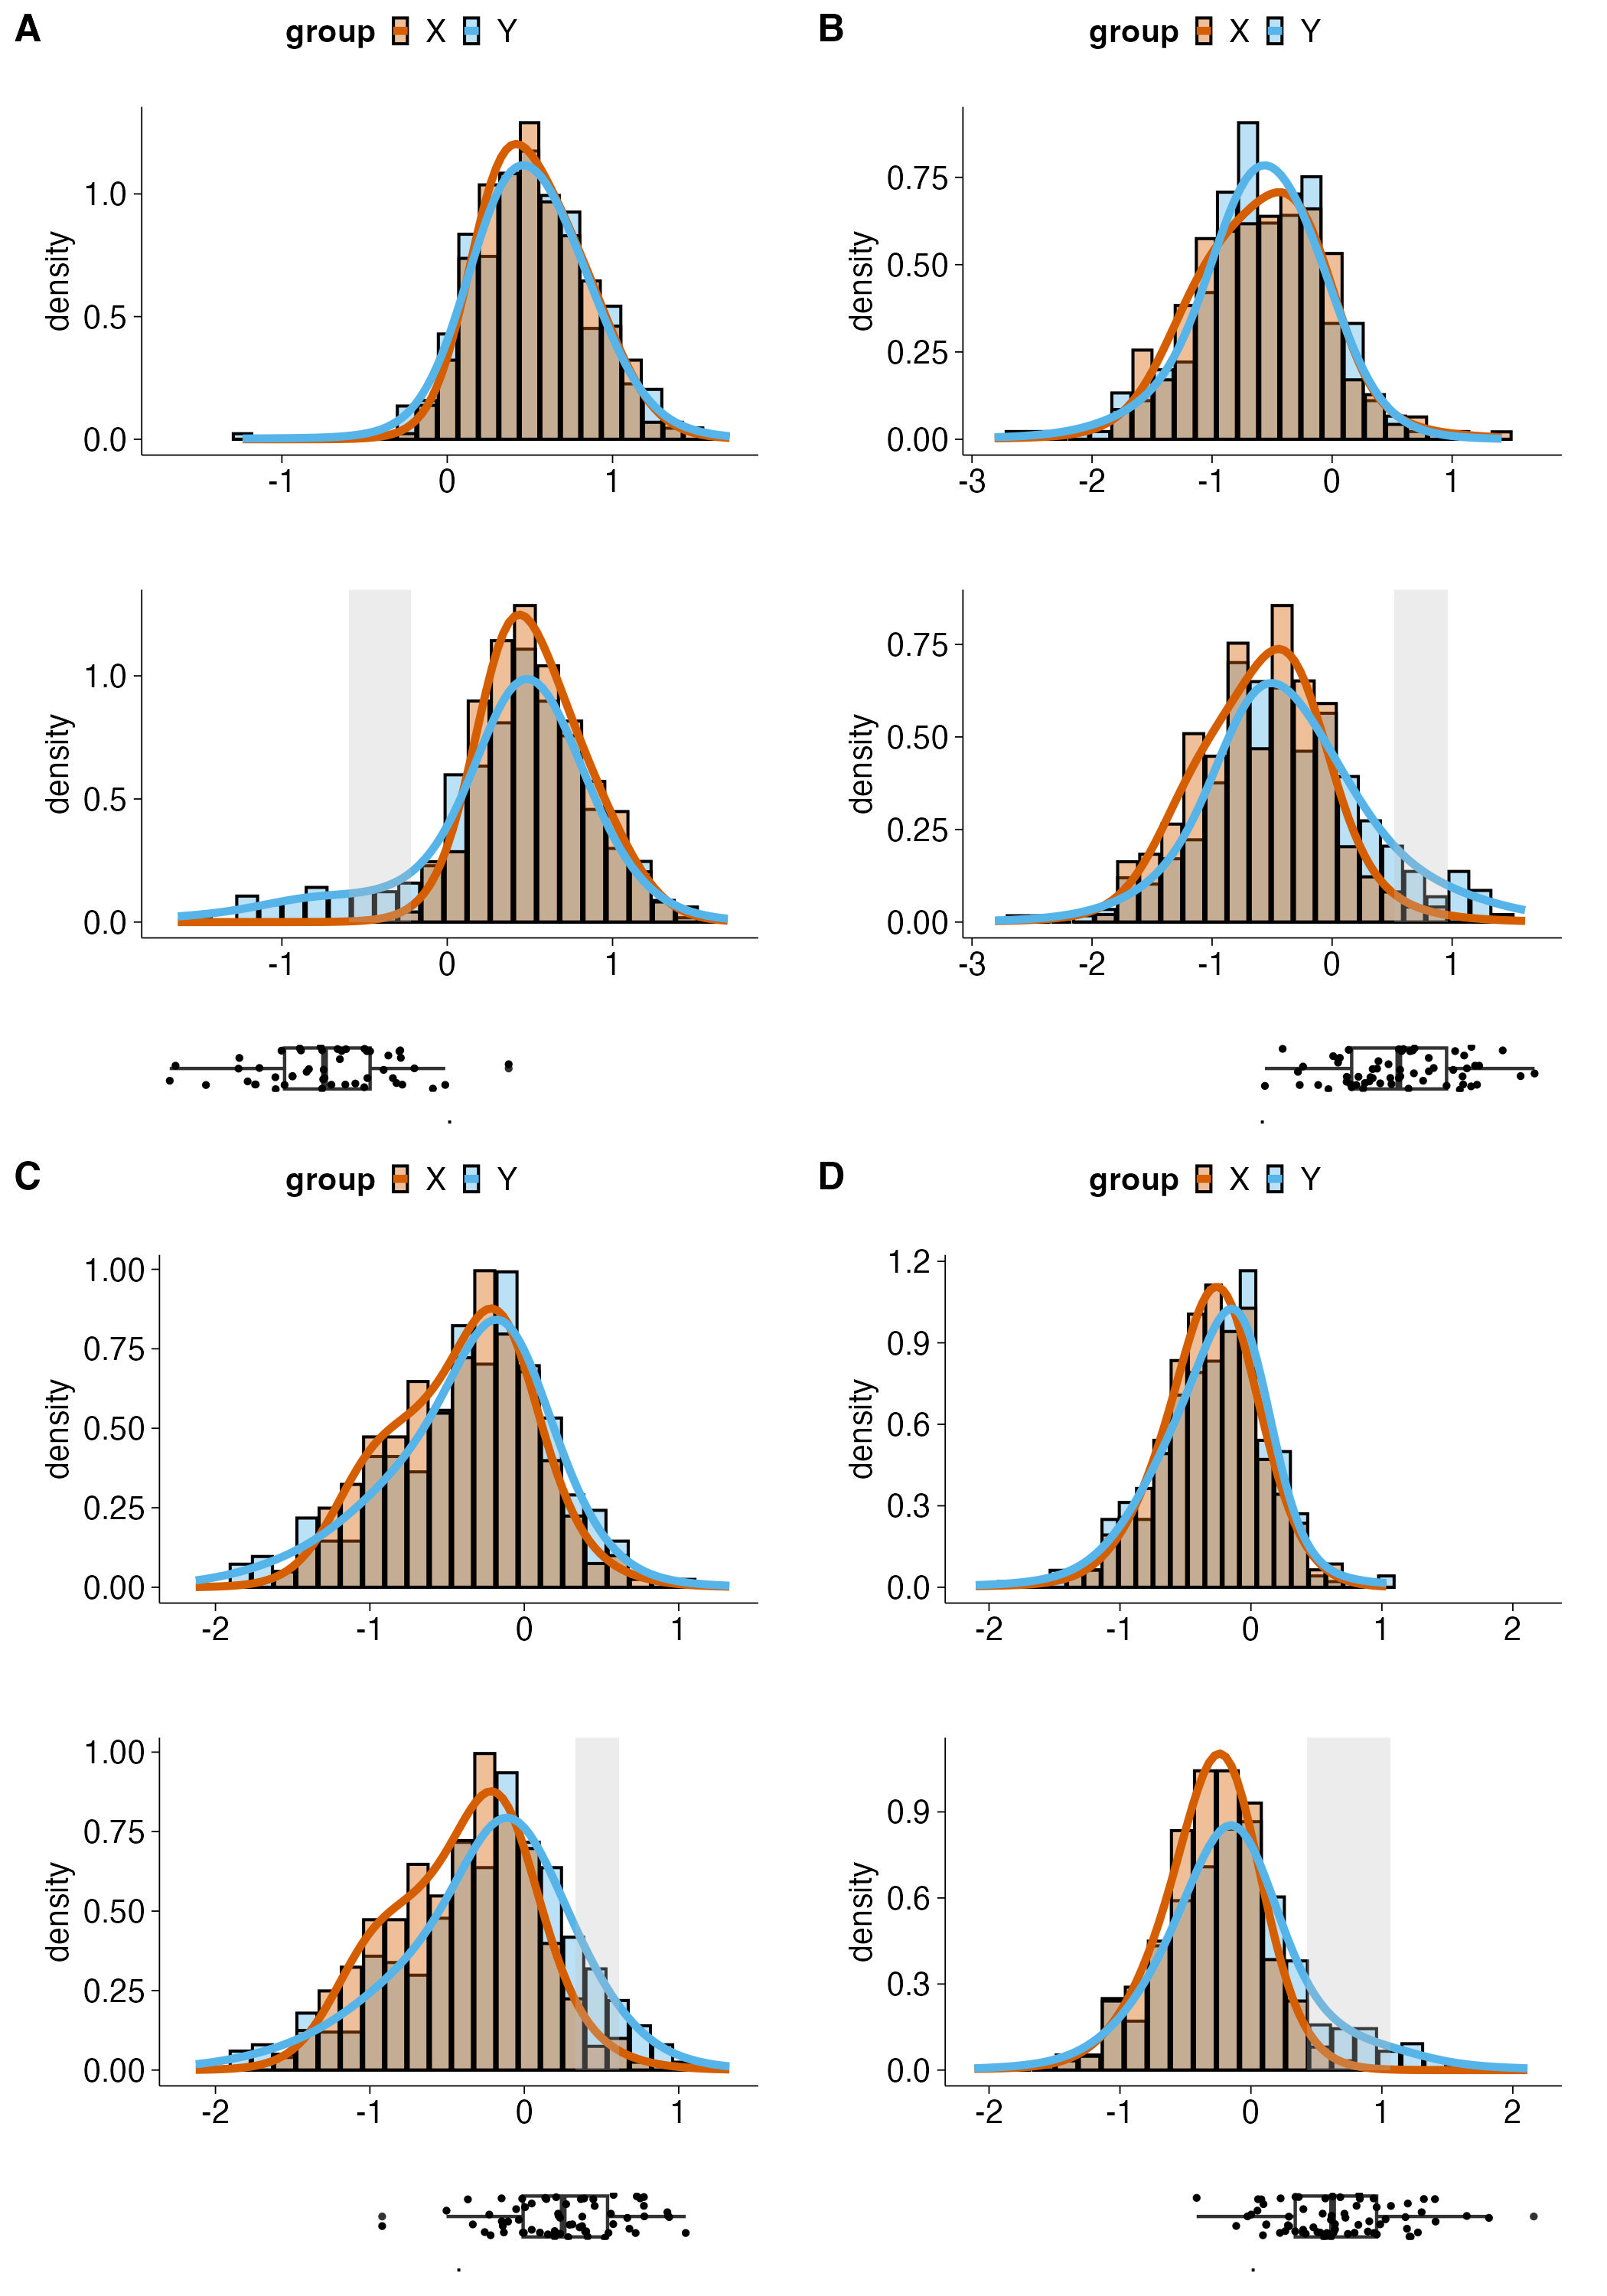
\includegraphics[width=0.85\linewidth]{figs/fig8.jpg}
    \captionsetup{labelfont={bf,small,color=red}}
    \caption{\textbf{\textcolor{red}{gamdid visualizations for four representative features detected by all three methods in the spike-in case study}} Each panel (\textbf{A}--\textbf{D}) shows one feature, following the same layout as the panels of Figure \ref{fig:msqrob_distinct_only}: the mock comparison (top), the comparison after spike-in (middle), and a boxplot indicating where the spike-in melanoma cells are located (bottom). All four features are detected as significant by msqrob2, gamdid, and distinct, forming part of the 52-feature consensus set (see Figure \ref{fig:volanoPlots}C). In all four cases, gamdid's visualization reveals that the distributional difference extends beyond a simple mean shift: these features are DD due to the subpopulation of spike-in cells rather than DA. Moreover, the spiked-in melanoma cells align closely with the detected differential region (gray shading) in each example. This demonstrates that even within the set of features identified by conventional DA methods, gamdid provides additional interpretive value by characterizing how and where the distributions differ. This information is not accessible from the fold change and p-value from a conventional DA method. These examples underscore the broader argument that accounting for full distributional differences, rather than mean shifts alone, leads to richer biological insights.}
    \label{fig:caseStudy_exs}
\end{figure}
